\documentclass[12pt]{book}
\usepackage{amssymb}
\usepackage{amsmath}
\usepackage{amsfonts}
\usepackage{tikz-cd}
\usepackage{stmaryrd}
\usepackage{hyperref}
\setlength{\evensidemargin}{0.25in}
\setlength{\oddsidemargin}{0.25in}
\setlength{\textwidth}{6in}
\parskip0.2em

\newtheorem{theorem}{Theorem}[section]
\newtheorem{lemma}[theorem]{Lemma}
\newtheorem{proposition}[theorem]{Proposition}
\newtheorem{corollary}[theorem]{Corollary}
\newtheorem{definition}[theorem]{Definition}
\newtheorem{conj}[theorem]{Conjecture}
\newtheorem{assumption}[theorem]{Assumption}
\newtheorem{property}[theorem]{Property}
\newtheorem{remark}[theorem]{Remark}
\newtheorem{example}[theorem]{Example}
\newtheorem{exercise}[theorem]{Exercise}
\numberwithin{equation}{section}
\allowdisplaybreaks[1]

%Peng's command
\newcommand{\MW}{Milnor-Witt\ }
\newcommand{\rMW}{\mathrm{MW}}
\newcommand{\KMW}{\mathrm{K}^\mathrm{MW}}
\newcommand{\KM}{\mathrm{K}^\mathrm{M}}
\newcommand{\sKMW}{\mathscr{K}^\mathrm{MW}}
\newcommand{\tbb}[1]{\widetilde{\mathbb{#1}}}
\newcommand{\wt}[1]{\widetilde{#1}}
\newcommand{\Spec}{\mathrm{Spec}\ }
\newcommand{\af}{\mathbb{A}}
\newcommand{\afnz}[1]{\mathbb{A}^{#1}\setminus \{0\}}
\newcommand{\nonZero}{\setminus \{0\}}
\newcommand{\cO}{\mathcal{O}}
\newcommand{\bZ}{\mathbb{Z}}
\newcommand{\bfZ}{\mathbf{Z}}
\newcommand{\tbZ}{\tbb{Z}}
\newcommand{\inv}{^{-1}}%
\newcommand{\Gm}{\mathbb{G}_m}
\newcommand{\tGm}{\tbb{G}_m}
\newcommand{\Sp}{\mathrm{Sp}}
\newcommand{\GL}{\mathrm{GL}}
\newcommand{\SL}{\mathrm{SL}}
\newcommand{\MSp}{\mathrm{MSp}}
\newcommand{\BSp}{\mathrm{BSp}}
\newcommand{\SH}{\mathcal{SH}}
\newcommand{\Da}{D_{\af^1}}
\newcommand{\Daba}[1]{D(Ab_{\af^1}(#1))}
\newcommand{\DM}{\mathrm{DM}}
\newcommand{\DMt}{\widetilde{\mathrm{DM}}}
\newcommand{\M}{\mathrm{M}}
\newcommand{\Mt}{\wt{\mathrm{M}}}
\newcommand{\Meta}{\wt{\mathrm{M}}_{\eta}}
\newcommand{\HH}{\mathrm{H}_{\rMW}}
\newcommand{\Heta}{\mathrm{H}_{\eta}}
\newcommand{\sBra}[1]{\left[#1\right]}
\newcommand{\aBra}[1]{\left<#1\right>}
\newcommand{\llBra}[1]{\llbracket #1 \rrbracket
}
\newcommand{\rHom}{\mathrm{Hom}}
\newcommand{\Ker}{\mathrm{Ker}}
\newcommand{\rFun}{\mathrm{Fun}}
\newcommand{\Spc}{\mathcal{S}pc}
\newcommand{\gy}{\rm{Gysin}}
\newcommand{\xr}[1]{\xrightarrow{#1}}

\newcommand{\AZ}{\mathbb{A}\mathcal{Z}}
\newcommand{\bfZa}{\mathbf{Z}_{\mathbb{A}^1}}
\newcommand{\tauO}{\tau^{\odot}}

\raggedbottom

\title{Seeing the Mountain}
\author{Keyao Peng}



\begin{document}
\begin{titlepage}
\begin{center}
{\huge\bfseries Seeing the Mountain \\}
% {\Large A Journey Through Post-Modern Geometry \\}
 % ----------------------------------------------------------------
 \vspace{1.5cm}
 {\Large\bfseries Keyao Peng}\\[5pt]
 keyao.peng@ube.fr\\[14pt]
  % ----------------------------------------------------------------
 \vspace{2cm}
 % ----------------------------------------------------------------
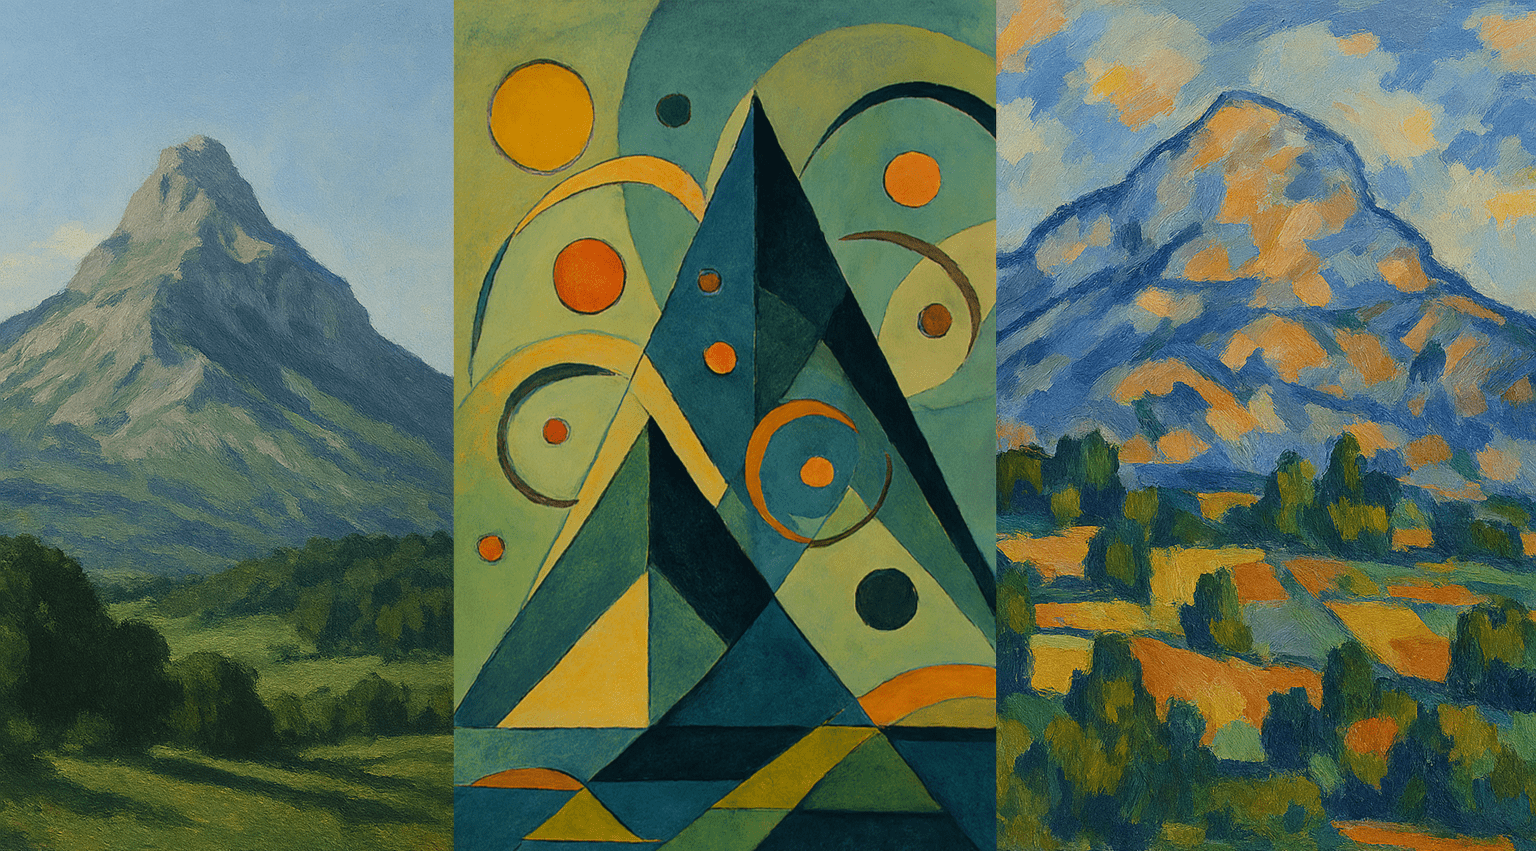
\includegraphics[width=\textwidth]{cover.png}\\[5pt]
 \vfill
{Sep 2025}
\end{center}
\end{titlepage}
\clearpage

\thispagestyle{empty}
\newlength{\longest}
\settowidth\longest{\huge\itshape Seeing the mountain still as a mountain.}
\null\vfill

\centering
\parbox{\longest}{%
  \raggedright{\huge\itshape%
  Seeing the mountain as the mountain; \\ 
  Seeing the mountain as not a mountain; \\ 
  Seeing the mountain as still a mountain. \par\bigskip
  }   
  \raggedleft\Large\MakeUppercase{Qingyuan Xingsi}\par%
}

\vfill\vfill

\clearpage

\tableofcontents

\chapter{Introduction}\label{chap:introduction}


\section{What is Algebraic Geometry?}

Algebraic geometry is the study of geometric spaces that locally arise as solutions to polynomial equations. This study can be approached at two levels:

\begin{itemize}
  \item \textbf{Local:} This involves studying the geometric properties of solution sets to polynomial equations. Since we work not only over $\mathbb{R}$ or $\mathbb{C}$ but potentially over arbitrary fields or rings, we must construct a more intrinsic notion of geometry associated with algebra—namely, the spectrum of a ring. This leads to the study of affine varieties and affine schemes, allowing a translation between algebra and geometry.

  \item \textbf{Synthetic:} Analogous to how manifolds generalize open subsets of $\mathbb{R}^n$, we study spaces that are locally isomorphic to affine varieties. This broader perspective leads to the study of varieties and schemes through various formal frameworks.
\end{itemize}

This lecture is part of an algebraic geometry course that emphasizes the second, synthetic level. However, the underlying question—“How can we construct and classify generalized spaces from certain building blocks?”—is relevant across many branches of geometry. Thus, this part can stand alone as a form of \emph{post-modern}\footnote{A commonly accepted definition is “after World War II.”} synthetic geometry.

\section{Essentialism vs. Structuralism}

Synthetic geometry formalizes geometric concepts through axioms that directly address fundamental entities—such as points and lines—rather than relying on a background space like Cartesian coordinates. In contrast to the analytic viewpoint, where every geometric object is composed of points, synthetic geometry treats lines, curves, and other entities as primitive. The focus shifts to the \textbf{relationships} between these objects, such as “a point lies on a line” or “two lines intersect.”

This structuralism perspective emphasizes understanding objects through their interactions. To formalize these relationships, we use \textbf{category theory} and \textbf{sheaf theory}. Moreover, by viewing categories themselves as spaces, we uncover deeper geometric structures. This formalism, developed through algebraic geometry, now plays a central role in various fields: differential geometry, topology, quantum field theory, and beyond.

\section{What is Geometry in Physics?}

Quantum physics connects to both the local and synthetic levels of algebraic geometry:

\begin{itemize}
  \item \textbf{Local:} The concept of the spectrum of a commutative ring originates from $C^*$-algebras and operator theory, both fundamental in quantum physics. The duality between algebra and geometry is already present in the Heisenberg and Schrödinger formulations.

  \item \textbf{Synthetic:} In quantum field theory, we study the space of field configurations (histories), which is infinite-dimensional and behaves irregularly. Nevertheless, we aim to treat it as a “manifold” to define metrics, path integrals, and differential forms. Synthetic geometry provides a rigorous framework for these constructions (e.g., via smooth sets). Gauge theory, supergeometry, and related topics can also be unified within this framework \cite{nlab:geometry_of_physics}.
\end{itemize}

A concrete example is mirror symmetry, which links Gromov–Witten invariants with Hodge theory.

\section{Course Plan}

We will focus on three types of geometry and study them comparatively using synthetic methods:

\begin{itemize}
  \item \textbf{Smooth Sets / Manifolds:} Built from open subsets of $\mathbb{R}^n$, these provide intuitive and geometric examples, serving as a bridge to classical geometry.

  \item \textbf{Simplicial Sets / Kan Complexes:} Constructed from simplices $\Delta$, these offer the simplest and most abstract examples.

  \item \textbf{Algebraic Sets / Schemes:} Built from spectra of commutative rings, these are the central objects of study in this course.
\end{itemize}


\bibliographystyle{plain}
\bibliography{references}
\end{document}
